\documentclass[useAMS,usenatbib]{mn2e}
\usepackage{aas_macros}
\usepackage[dvips]{graphicx}
\usepackage{amssymb,amsmath}
\usepackage{times}
\bibliographystyle{mn2e}
%\documentclass[a4paper,10pt]{article}
%
%
\begin{document}
%
\title[Correlations between DM, Gas, Star Components]
      {Correlations between Dark Matter, Gas and Star Components of Halos in
        SPH Simulations}
% original title: Quantification of Angular Momentum Disalignment
% between Dark Matter Halos and Baryonic Gas
\author[P. Steger et al.]{Pascal S. P. Steger$^{1}$\thanks{E-mail: psteger@phys.ethz.ch},
  Oliver J. Hahn$^{2}$,
  C. Marcella Carollo$^{1}$,
  Cristiano Porciani$^{3}$\newauthor
  and Giuseppe Tormen$^{4}$\\
  $^{1}$Department of Physics, ETH Z\"urich, CH-8093 Z\"urich,
  Switzerland\\
  $^{2}$KIPAC, Stanford University, 2575 Sand Hill Road, Menlo Park,
  CA 94025, USA\\
  $^{3}$Argelander-Institut f\"ur Astronomie, D-53121 Bonn, Germany\\
  $^{4}$Dipartimento di Astronomia, Universit\`a di Padova,
  Vicolo dell'Osservatorio 2, I-35122 Padova, Italy }
%
%
\date{\today}
\pagerange{\pageref{firstpage}--\pageref{lastpage}} \pubyear{2010}
\maketitle
\label{firstpage}
\begin{abstract}
  We quantify disalignment of angular momentum between gas, stars and dark
  matter components of halos in cosmological SPH-simulations in
  $\Lambda$CDM. Furthermore, we investigate correlations between angular
  momentum, inertia axes and the eigenvectors of the tidal field. These
  correlations will help to constrain contamination of weak lensing signals
  arising due to intrinsic alignment. The spin-parameter distributions with
  distinction between the three particle types and velocity dispersions allow
  us to estimate the influence of ordered rotation on these correlations.

  We find:
%
  (1) a median angular momentum disalignment of $76^\circ$ between the gas and
  the dark matter component and of $59^\circ$ between stars and dark matter;
%
  (2) a correlation between the biggest eigenvector $\mathbf{t}_1$ of the
  tidal field and total angular momentum that is similar, but less distinct
  than between $\mathbf{t}_1$ and the main inertia axis;
%
  (3) the halo spin parameter of gas to be roughly an order of magnitude
  higher than the one of dark matter and stars.
\end{abstract}
%
\begin{keywords}
  cosmology: theory, large-scale structure of Universe --
  %galaxies: formation, evolution --
  methods: numerical
\end{keywords}
%
%
\section{Introduction}
\label{chap:intro}
%
%% CONTEXT
%
To describe the universe and its temporal evolution, to find the dark matter
distribution and thereby to follow the galaxy formation history is the
long-term goal of extragalactic astronomy.
%
%% SIMULATIONS
%
\begin{figure}
% should show up on first page
  \begin{center}
    \includegraphics[width=0.45\textwidth]{fig/splotch/out.eps}
  \end{center}
  \caption{ \label{fig:splotch} Visualization by ray-tracing of one of the
    resimulated clusters. The visible box size spans a range of $50\,h^{-1}{\rm
      Mpc}$.}
\end{figure}
%
%
By starting from visible parts of galaxies, gas and stars, one has to infer
all properties used in the overall description as e.g. mass, shape parameters
and angular momentum. Using simulations one starts with a known distribution
of dark matter, gas and stars and infers properties from them that can be used
as predictions for observations.
% resolution issue: either high resolution, galaxy scale
%                   or low resolution, large scale
The available resources restrict the achievable resolution: If one wants to
sample the matter distribution with high resolution, only relatively small
scales are sampled; on the other hand there is only coarse resolution when
working on the largest scales.
% trick: resimulation
Resimulations do circumvent this restriction partly: After a low resolution
run on large scales an interesting region is selected and traced backwards to
the initial conditions, which are resampled to higher resolution. The
surroundings are kept at low resolution, thus providing the same large scale
influence, but at lower computational cost. Figure \ref{fig:splotch} shows a
snapshot of a resimulated cluster at $z=0$, rendered with {\sc
  Splotch}\footnote{http://dipastro.pd.astro.it/~cosmo/Splotch}. Colors encode
the internal energy of the gas particles, star density gives intensity.

%
%
%% PROPERTIES under consideration
%
%% SHAPE
%
One of the observable properties of galaxies that first spring into mind is
its shape. In order to connect the measured shape of the baryons with the
shape of the more influential dark matter part, we investigate the alignment
of halo shape parameters with each other.

The temporal evolution of the shape is given, as pointed out by
\cite{Valluri2010}, by adaptions of individual particle orbits to the changing
potential. The potential is changed by encounters with neighboring halos or by
interaction with the large scale structure. All changes in particle orbits
affect the angular momentum, which in turn can be observed from the rotation
of the baryonic matter in the center of the halo. In this article we
investigate alignments of shape parameters of components of the halo with each
other as well as with angular momentum and the large scale structure.

It has been established by observations and reproduced in simulations that
there are a number of significant alignments, indeed: In gravitational
potentials of clusters, gas traces the shape of the dark matter halo pretty
well outside the core (\cite{Lau2010}). Further away, it is found that the
major axes of subhalos align with the direction to the center of mass of the
respective host halo (\cite{Yang2006}, \cite{Faltenbacher2007},
\cite{Faltenbacher2008}), indicating a contribution from small scale
gravitational influence. On bigger scales, \cite{Wang2008} found alignments
between the major axes of host galaxies in neighboring groups as well as
impact on the alignments of satellites. \cite{Aragon-Calvo2007} indicate that
the minor axes tend to lie perpendicular to the host structure. On the very
biggest scales, \cite{Basilakos2006} find an alignment between cluster and
supercluster major axes, while \cite{Cuesta2008} report that halos on the
shells of voids preferentially align their angular momentum and shape
perpendicular to the direction joining halo and void center.

%
%% ANGULAR MOMENTUM
% searching connection with dynamical property
% quite basic stuff, check/delete !
In order to understand the evolution of galaxies one has to account for the
buildup of dynamical properties as e.g. angular momentum. \cite{Peebles1969}
showed that the angular momentum observed nowadays agrees with galaxy
formation through gravitational instability. Starting from Gaussian initial
conditions at early time, tidal torques of large scale structures induce
torquing on smaller structures and seed the first buildup of angular momentum,
see e.g. \cite{Barnes1987} for simulations with different initial conditions.

The contributions to angular momentum by dark matter, gas and stars differ
considerably:

Angular momentum of dark matter is mainly conserved; simulations performed by
e.g. \cite{Sharma2005} indicate that roughly half of the dark matter is
rotating in the same sense as baryonic matter, while the other half is
counterrotating.

The fact that a net angular momentum is observed in galaxies suggests that
there exists a process to enhance angular momentum for stars and gas. The
configuration with smallest energy for a selfgravitating system with given
angular momentum is a disk, which is observed in late type galaxies, after a
big amount of internal energy of the gas is radiated away. Stars in elliptical
galaxies have left the disks due to orbit instabilities encountering external
gravitational influences. Violent relaxation then leads to the observed number
density distribution; the angular momentum in the central parts of halos is
increased by transferring some small fraction of the halo mass outwards.

With numeric simulations, one tries to quantize the history of angular
momentum buildup and transformation between the different components.
%
\cite{Sharma2005} investigate the angular momentum disalignment of the gas and
dark matter components of halos in a nonradiative $N$-body/SPH simulation and
find a misalignment of typically $20^\circ$. \cite{Croft2008} included
disalignments between star and dark matter components in the analysis at $z=1$
and found median values of $43.5^\circ$ for stars and $69.6^\circ$ for
gas. With a simulation up to $z=0$, we are able to compare with the previous
results and search for depences on halo mass.
% disalignment between host/subhalo
Halos in the near vicinity of larger halos experience gravitational forces
that influence their orientation, e.g. by precession. As subhalos fly by the
core of their host, they reorient themselves with respect to its center, given
that the typical rotation timescale is smaller than the time to cross the big
structure. See \cite{Pereira2008} for a reference. This work quantifies
alignment between particle types as function of radial separation, measured in
terms of the virial radius of the host.

%weak lensing
% contamination from large scale gal-gal ellipticity al
% contamination from shear-ellipticity al
The distribution of the disalignment angle as found in numerical simulations
e.g. by \cite{VanDenBosch2002} leave an imprint on the measured intrinsic
alignments that attribute to weak lensing signal. This is used in future
high-precision studies of dark energy, see e.g. \cite{Catelan2001} for the
contamination from large-scale alignments with ranges of $1$ to $100\rm{Mpc}$
and \cite{Hirata2004} for the shear-ellipticity alignment. Estimates for
intrinsic alignments as function of redshift and environment therefore help to
deduce the large scale structure of dark matter from observations.
%
%%ENVIRONMENT
% web: void, sheet, filament, cluster
The environment in which a halo resides is part of the cosmic web: vast
regions called voids with low density, embedded in sheets of higher density at
their borders, which meet in filaments which in turn are connected by dense
clusters (cf. \cite{Tegmark2004} for two galaxy surveys, \cite{Shandarin1989},
\cite{Bond1996}). This cosmic web follows from Gaussian perturbations in the
early stage of the universe through collapse along the main axes of the strain
tensor, cf. \cite{Zel'Dovich1970} for a first order approximation.

% alignment with void dir, filament, to clusters
\cite{Brunino2007} and \cite{Cuesta2008} report on a mean alignment between
the angular momentum and the radial direction to the nearest void in numerical
studies. \cite{Hahn2010} quantify the alignments of halos inside a filamentary
structure at redshifts $z=1,0.5,0$. They find that massive galaxy disks have
spins aligned with the filament.
%
%%TIDAL FIELD
%
To measure this kind of alignment, one has to consider the structure of the
tidal field. Its imprint on the orientation of the galaxies today is best
described by tidal torque theory, which gives expressions for the two-point
correlation function of the tidal field (\cite{Porciani2002a},
\cite{Porciani2002b} and references). \cite{Schaefer2008} gives an overview of
the connections between tidal torquing and angular momentum aquisition as well
as the resulting angular momentum distribution. With our work we are able to
probe alignments of the baryonic parts of the galaxies with the tidal field on
arbitrary scales, concentrating on $1\,h^{-1}{\rm Mpc}$.

%% ORGANIZATION OF PAPER
%
The rest of the paper is laid out as follows: Chapter \ref{chap:data} gives an
overview over the specifications of the simulations under consideration;
definitions and methods are laid down in chapter \ref{chap:defs}. In chapter
\ref{chap:res} we present our results for the disalignment between angular
momentum, main inertia axis and tidal field eigenvectors. It follows a summary
in chapter \ref{chap:disc}; we conclude the work with propositions for further
investigations. The appendix contains comparisons of the two calculation
methods given by our definitions and {\sc Ahf}, while checks for numerical and
statistical artefacts are described directly with the results.
%
%
\section{The Data}
\label{chap:data}
%
\subsection{Specifics of the Simulations}
%
%
We use high-resolution cosmological hydrodynamic simulations of three
individual galaxy clusters -- see figure \ref{fig:splotch} for a visualization
of a low-resolution run of cluster 3 -- embedded in a cosmological box of
$192\,h^{-1}{\rm Mpc}$. The cosmological model assumes a flat $\Lambda$CDM
cosmology with matter density parameter $\Omega_m =0.3$, baryon fraction
$\Omega_b=0.04$, Hubble constant $H_0=hH_{100}=70\,{\rm km}\,{\rm
  s}^{-1}\,{\rm Mpc}^{-1}$ and a power spectrum normalization of
$\sigma_8=0.8$. The simulations were performed using the tree-SPH+$N$-body
code {\sc Gadget-2} \citep{Springel2005} and include subgrid models for
cooling, star formation and stellar feedback identical to the simulations
described by \cite{Borgani2004}. AGN feedback is not included, so the density
inside the halo centers is enhanced due to overcooling. As shown by
\cite{Sales2010} recently, this effect increases the mass of a halo by a
factor $\pm10$. The angular momentum of the galaxy being roughly half the one
of the surrounding halo is however largely independent of halo mass and
feedback scheme. We conclude that angular momentum and principal axes are not
considerably changed.

The three galaxy clusters were resimulated at 45 times higher resolution
giving a mass resolution of $1.03\times 10^{7}\,h^{-1}{\rm M}_\odot$ for the
dark matter component, while gas and stars were both sampled with particles of
mass $7.7\times 10^6\,h^{-1}{\rm M}_\odot$. Dark matter particles in the
outskirt of the simulation box have varying masses above $5.33\times
10^9\,h^{-1}{\rm M}_\odot$. Spatial smoothing is performed over a Plummer
equivalent's width of $7.5\,h^{-1}{\rm kpc}$.

All simulations started at $z=100$ and evolved until $z=0$ where we perform
the analysis. The properties of the three resimulated clusters at $z=0$ are
summarized in table \ref{tab:clusterprop}.
%
\begin{table}
  \begin{center} \begin{tabular}{lcccc} \hline Simulation &
      $M_{\rm vir} / h^{-1}{\rm M}_\odot $ & $R_{\rm vir} /
      h^{-1}{\rm Mpc}$ & $N_{\rm sub}$ & $N_{\rm field}$ \\ \hline
      c1 & $2.8900\times10^{14}$ & 1.3466 & 502 & 218 \\ c2 &
      $1.6021\times10^{14}$ & 1.1062 & 279 & 200 \\ c3 &
      $2.4922\times10^{14}$ & 1.2817 & 399 & 163 \\ \hline
    \end{tabular} \end{center}
  \caption{\label{tab:clusterprop}Properties of the resimulated
    clusters. $M_{\rm vir}$ and $R_{\rm vir}$ are the virial mass and radius
    of the clusters. The number of subhalos above $M=5\cdot10^9h^{-1}{\rm
      M}_\odot$ within the cluster virial radius is given by $N_{\rm sub}$,
    while $N_{\rm field}$ is the number of isolated halos above
    $M=5\cdot10^9h^{-1}{\rm M}_\odot$ within $3$ virial radii from the cluster
    center.}
\end{table}
%
\subsection{Halo and Subhalo Samples}
%
Halos and subhalos in the high-resolution region were identified with the {\sc
  Amiga} halo finder (\cite{Knollmann2009} and \cite{Gill2004a}) that
identifies a hierarchy of gravitationally bound density peaks:

Starting from local density minima or leaves of a adaptive mesh refinement
hierarchy all particles in a sphere around this point are included, out to a
radius where the density falls below $\Delta{\rm vir}\bar{\rho}$, as defined
by \cite{Bryan1998}. Additionally, particles residing in a lower density
environment -- or equivalently in a higher level in the AMR tree -- are
assigned to the nearest halo of the same level. The halo edge is determined as
the contour at which the density starts to rise again. Particles that happen
to lie in the realm of a halo but are not gravitationally bound are removed
iteratively; the halo properties are calculated from the remaining sample, by
integrating over logarithmically spaced shells centered on the center of mass.

% additional unbinding procedure
In order to treat near encounters correctly, where we center on the most bound
particle instead on the center of mass, we implemented an additional procedure
to remove still unbound particles iteratively, as proposed by
\cite{Porciani2002a}: The most unbound particle is excluded, potential and
kinetic enrgy get recomputed, then the next most unbound particle is searched
for. Excluded particles are allowed to reenter the halo at a later step if
they get bound again. A mean fraction of 3\% of the particles is excluded in
addition to the unbinding procecure from {\sc Amiga} in the low resolution
run; the main contribution coming from low mass halos, as the gravitational
potential generated from particles outside the virial radius is completely
neglected by such an approach. We find that contamination from a few virially
unbound particles -- especially gas particles with too high internal energy --
is less important than the error induced from lower particle numbers for the
smaller halos and the gas and star components with low resolution. Therefore,
the procedure is not invoked for computations including gas and star
particles.

We computed the complete subhalo tree using {\sc MergerTree} to find particles
shared by several halos in the same simulation snapshot and searching the
respective host halo as the one which owns the highest fraction of particles
residing in a given halo.

%
A total of $11\%$ of the halos are assigned to a host halo; all other halos
are considered single halos. Searching for correlations between subhalos and
their host we analyze the properties of these single halos with respect to the
halo residing in the cluster center of each simulation and afterwards stack
the resulting values for analysis.

% stacking, constraints for halos to be considered
For each halo we determine the shape and angular momentum of gas, stars and
dark matter as described in the next chapter. If not specified otherwise, the
figures were created using particles of all types together. For our analysis,
we stack the halos of all three clusters and restrict ourselves to halos that
have more than $200$ dark matter, more than $10$ gas and star particles
inside. Moreover, we exclude all halos that contain low resolution dark matter
particles with a mass bigger than $1\%$ of the halo mass. This exclusion
mainly applies for small halos in the outer regime of the simulation box where
low resolution particles -- with an overall occurrence of only $0.07\%$ -- can
dominate determination of the halo properties.
%
%
\section{Definitions}
\label{chap:defs}
%
\subsection{Shapes}
%
The shape of a halo with $N$ particles is determined by its weighted moment of
inertia tensor (see e.g. \cite{Hahn2007a}, \cite{Porciani2002a}),
%
\begin{equation} \label{eq:Idef}
  I_{jk}\equiv\sum_{i=1}^N m_i(r_i^2\delta_{jk}-(x_i)_j(x_i)_k)
\end{equation}
%
with the distance $r_i\equiv((x_i)_1,(x_i)_2,(x_i)_3)$ of a particle at
position $x_i$ from the center of mass. Written in an eigensystem with
eigenvectors $\mathbf{e}_1,\mathbf{e}_2,\mathbf{e}_3$, it reads as
%
\begin{equation} \label{eq:Ieigen}
  \tilde{I}=\frac{M}{5}\cdot\rm{diag}
  (\ell_1^2+\ell_3^2, \ell_1^2+\ell_3^2, \ell_1^2+\ell_2^2)
\end{equation}
%
with the lengths of the pricipal axes $\ell_1\geq\ell_2\geq\ell_3$. All
computations of correlation functions use the corresponding eigenvectors
normalized to 1, while the degeneracy stemming from multiplication of -1 is
removed using absolute values.
%
\subsection{Angular Momentum}
%
The classical definition of
%
\begin{equation} \label{eq:AngMom}
  \mathbf{J}\equiv\sum_{i=1}^N \mathbf{r}_i\times m_i\mathbf{v}_i
\end{equation}
%
is used to calculate the angular momentum in the center of mass frame. The sum
in (\ref{eq:AngMom}) goes over all bound particles of the halo, out to the
virial radius. We note that particles with a mass fraction of $8.5\%$ are
excluded by a spherical overdensity criterion in comparison with all particles
assigned to the respective halo.

{\sc Amiga} uses a slightly different method with averaging over concentric
shells around the center of mass with logarithmic spacing, resulting in a
slightly higher value for the angular momentum. We use the classical sum, as
the radius from the center of mass is computed for each particle separately.

An additional quality improvement that we shall include in a future work is
inclusion of bound particles outside the sphere of $\rho > \Delta(z)\rho_{\rm
  mean}$.
%
\subsection{Halo Spin Parameter}
%
Following \cite{Bullock2001}, we define the spin parameter
%
\begin{equation}\label{eq:lprime0}
  \lambda'\equiv\frac{|\mathbf{J}|}{\sqrt{2}MRV}
\end{equation}
%
with the angular momentum $\mathbf{J}$ inside a sphere of radius $R$, mass $M$
and circular velocity $V$. We have $V^2=GM/R$ if the halo is in dynamical
equilibrium and therefore
%
\begin{equation} \label{eq:lprime1}
	\lambda'=\frac{|\mathbf{J}|}{\sqrt{2GR}M^{3/2}},
\end{equation}
%
where $J$ and $M$ are calculated from particles inside a sphere around the
most bound particle, with radius $R_{\rm vir}$. Inside this sphere
$\rho<\Delta(0)\rho_{\rm crit,0}$, with $\Delta(z)$ given by \citep{Bryan1998}
%
\begin{align} \label{eq:Deltaz}
	\Delta(z)&=18\pi^2+82f(z)-39f^2(z)\\
	f(z)&=-\frac{\Omega_\Lambda}{\Omega_m(1+z)^3+\Omega_\Lambda}
\end{align}
%
\cite{Bullock2001} established that $\lambda'_{\rm DM}$ is best described by a
log-normal distribution,
%
\begin{equation} \label{eq:plambda}
  p(\lambda)d\lambda=
  \frac{1}{\sqrt{2\pi}\sigma_\lambda}
  \exp\Bigl[-\frac{\ln^2(\lambda/\bar{\lambda})}{2\sigma_\lambda^2}\Bigr]
  \frac{d\lambda}{\lambda},
\end{equation}
%
which is a simple parabola $y=ax^2+bx+c$ in a logarithmic plot. This
distribution is found to be robust under varying measures for the radius of
the sphere. We use the same definition for gas and star components.
%
\subsection{Rotation support}
%
Rotationally supported spherical systems can be distinguished from systems
with random motion by the ratio $\Sigma/V_{\rm rot}$, with the velocity
dispersion
%
\begin{equation} \label{eq:sigma}
	\Sigma = \sqrt{\sum_{r_i<R_{\rm vir}}
			 \langle v_i^2\rangle-\langle v_i\rangle^2}
\end{equation}
%
and the rotation velocity $V_{\rm rot}$ of the particles in dynamical
equilibrium at the virial radius from the halo center. The lower the velocity
dispersion with respect to the virial velocity, the more particles move in the
same manner and hence the bigger is the rotation support.
%
%
\subsection{Tidal Field}
%
We compute the local eigenstructure of the smoothed tidal field tensor at the
position of each halo in order to probe the alignment with the large-scale
structure \citep[cf.][]{Hahn2007b}. First, we solve Poisson's equation by Fast
Fourier Transform on a grid of $512^3$ cells for the smoothed overdensity
field $\delta=\rho/\bar{\rho}-1$ by the double convolution $\phi_R =
\delta\star W_R\star G$, where $G$ is the Green's function of the symmetric
3-point finite difference operator and $W_R$ is the window function of scale
$R$ used to smooth the density field, top hat or Gaussian. The tidal tensor
%
\begin{equation}
  T_{ij}(\mathbf{x}) \equiv
  \left[\partial_i\partial_j-\frac{1}{3}\,\delta_{ij}\nabla^2\right]
  \phi(\mathbf{x})
  \label{TidalField}
\end{equation}
%
is then evaluated at the positions of the halo centers by finite
differencing. We finally compute eigenvalues $\tau_1\leq\tau_2\leq\tau_3$ and
corresponding eigenvectors $\mathbf{t}_1,\mathbf{t}_2,\mathbf{t}_3$ for each
halo. Halos with three positive eigenvalues correspond to clusters, filaments
have one negative eigenvalue, sheets two and voids with unstable orbits have
no positive eigenvalues.
%
\subsection{Angle}
We measure the angle between two vectors $\mathbf{p},\mathbf{q}$ by its
cosine,
%
\begin{equation}
  \phi(\mathbf{p},\mathbf{q})\equiv
	\frac{\mathbf{p}\cdot\mathbf{q}}{|\mathbf{p}|\cdot|\mathbf{q}|}.
\end{equation}
%
Eigenvectors of the inertia tensor after normalization are degenerate up to a
factor $\pm1$. When correlating them with other vectors, we therefore will use
the absolute value of $\phi$.
%
%
\section{Results}
\label{chap:res}
%
\subsection{Subhalo Mass Function}
%
%%%fig:shmf
%
\begin{figure}
  \begin{center}
    \includegraphics[width=0.45\textwidth]{fig/shmf/out.eps}
  \end{center}

  \caption{ \label{fig:shmf} Differential subhalo mass function incorporating
    all particle types, $\log_{10}p(m/M)\propto dn(m/M)/d\log_{10}m/M$, where
    $m$ is the mass of the subhalo, $M$ of its host. }
\end{figure}
%
%
The differential subhalo mass function as shown in figure \ref{fig:shmf} is in
good agreement with a power law of slope $-1$, cf. \cite{DeLucia2004}. Note
that all subhalos with mass $m$ of a host halo of mass $M$ such that
$\log_{10}(m/M)<-4$ are excluded: below this threshold the discreteness of the
halo constituents and their composition of particles with different masses
imply that too little subhalos of a given mass are counted.
%
%
\subsection{Shape: Sphericity}
%
%%%fig:aoverc
%
\begin{figure}
  \begin{center}
    \includegraphics[width=0.45\textwidth]{fig/aoverc/out.eps}
  \end{center}

  \caption{ \label{fig:aoverc} Inverse sphericity $\ell_1/\ell_3$. Blue points
    represent values from {\sc Ahf}, red points correspond to values computed
    with our framework. See text for further explanations.}
\end{figure}
%
%
In figure \ref{fig:aoverc} we have plotted the distribution of the inverse
sphericity $1/S=\ell_{1}/\ell_{3}$. Strictly spherical systems with $a\approx
c$ are slightly depressed, over all bins starting from the second we are
consistent with a power law of slope $-5.4\pm0.3$.  We have plotted the
results of our framework as well as the results from {\sc Amiga} as an example
for the correspondances and the differences between both calculation
methods. These are discussed further in the appendix. For highly nonspherical
systems the difference between center of mass (as used by {\sc Amiga}) and the
position of the most bound particle (as used by our framework) begin to
differ, mainly for halos with lower resolution.
%

\subsection{Shape: Radial Dependence}
%
%%%fig:rea
%
\begin{figure*}
  \begin{center}
    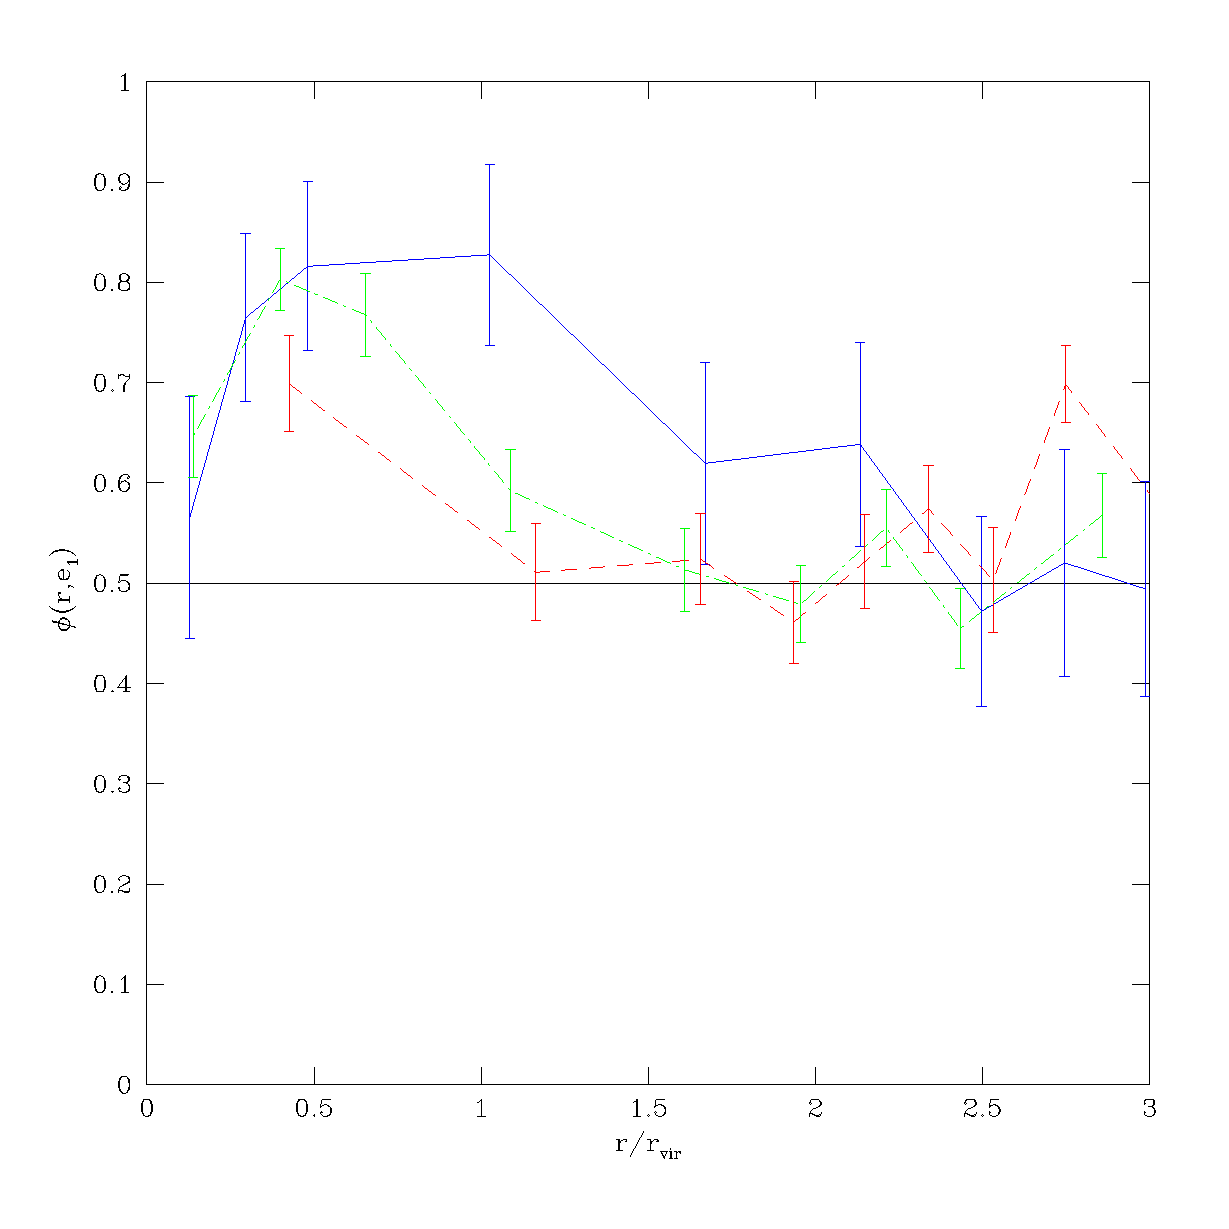
\includegraphics[width=0.45\textwidth]{fig/rea/outbig.eps}
    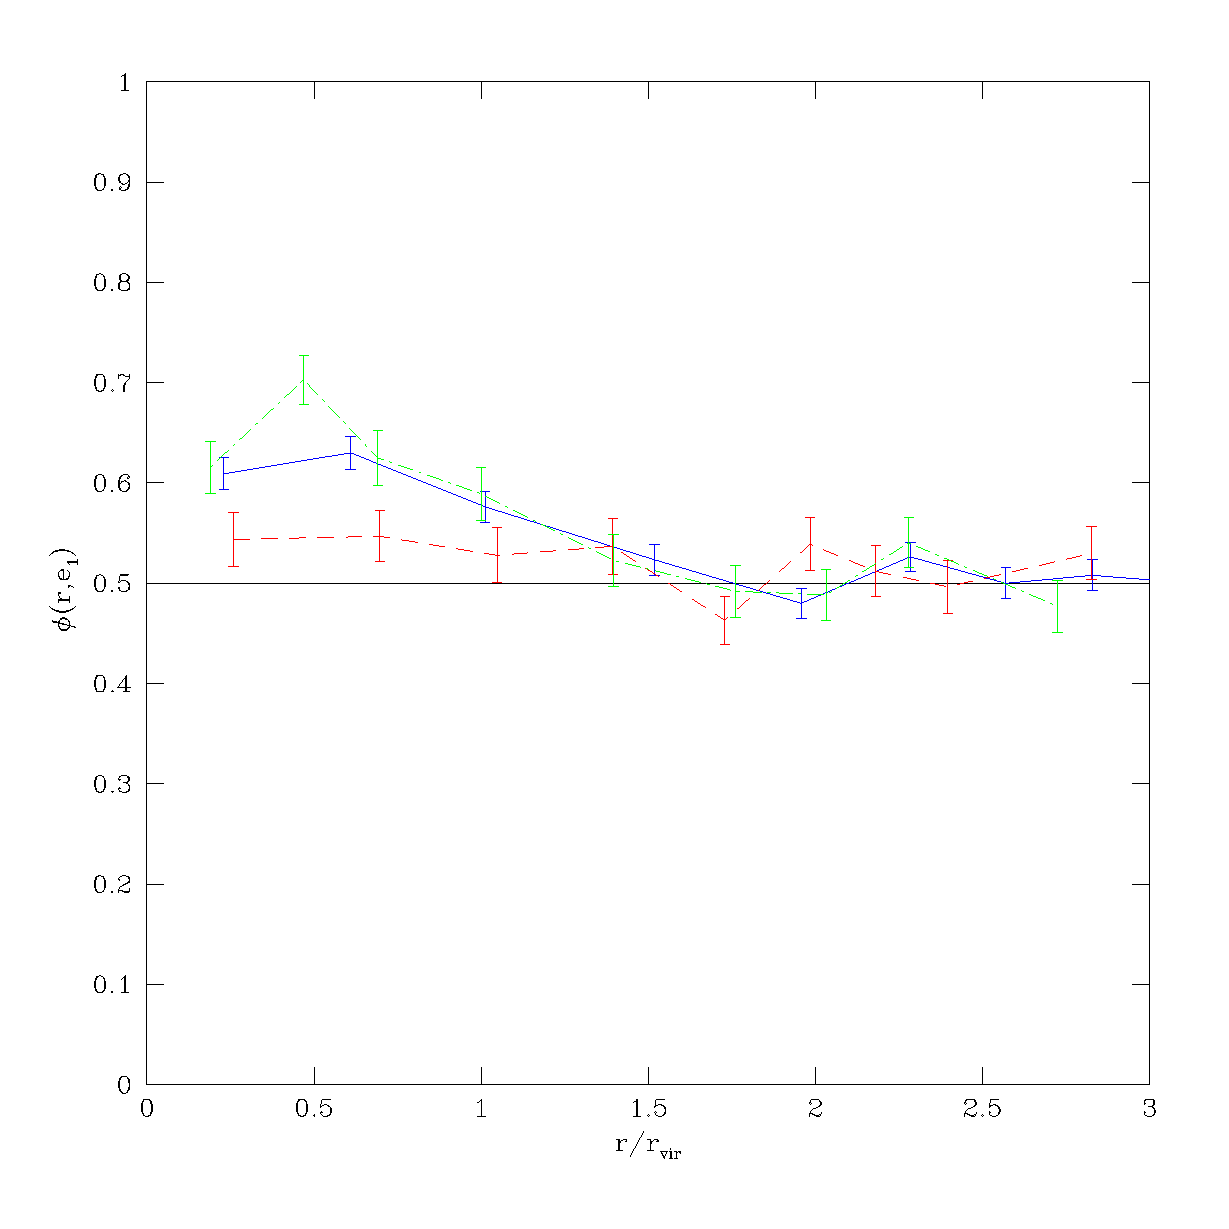
\includegraphics[width=0.45\textwidth]{fig/rea/outsmall.eps}
  \end{center}

  \caption{ \label{fig:rea} Distance dependence for the alignment between the
    main inertia axis $\mathbf{e}_1$ and the radial vector $\mathbf{r}$ to the
    cluster center. Panels on the left side include all halos with mass
    $m\geq10^{11}{\rm M}_\odot$, panels on the right side take all halos into
    account with $m<10^{11}{\rm M}_\odot$. Dark matter, gas and stellar
    components are shown in blue, red and green color.}
\end{figure*}
%
%
Figure \ref{fig:rea} presents the radial alignment of the main inertia axis of
the dark matter component with the radial vector as function of distance, as
investigated previously by \cite{Pereira2008} in dark matter only simulations.

Two mass bins with all halos above and below $M=10^{11}h^{-1}M_{\odot}$ are
shown. The splitting point in mass is chosen such that all halos with smaller
mass do not host a hot pressurized atmosphere that exerts ram pressure on the
central galaxy (\cite{Hahn2010} and references).

We recover the expected behavior for dark matter in the low mass range
($m<10^{11}{\rm M}_\odot$), and find an even stronger correlation with a
maximum around $r\gtrsim R_{\rm vir}$ for the high mass range; at radii higher
than $2R_{\rm vir}$ the distribution is not significantly differing from an
isotropic distribution with $\phi(\mathbf{r},\mathbf{e}_1)=0.5$.

Gas in high mass halos follows the trend for alignment at distances smaller
than the virial radius of the host, but fails to maintain this alignment
outside the virial radius. The upturn at $r/r_{\rm vir}>2$ is produced
possibly by massive halos in the outskirts of the cluster, as the exclusion
criterion for gas restricts the analysis to massive halos, while most of the
halos with large $r/r_{\rm vir}$ are analyzed with respect to the cluster
center. Ideed, the low mass sample shows no significant upturn in these
regimes.

Stars show a distinguished peak at low mass, which decays with distance out to
$r/r_{\rm vir}=2$. Surprisingly, it shows stronger alignment than dark matter
at small distances; in the high mass regime, this trend is not observed. We
suggest that the creation of star particles at relatively late times, when
there exists a pronounced environment, lets them feel the influence on small
scales more strongly than the surrounding dark matter halo; this effect seems
to be stronger for low mass halos, as indicated by the fact that dark matter
in the high mass sample follows this trend out to an even larger radius.

\subsection{Kinematics: Spin parameter}
%
%%%fig:lprime_dgs
%
\begin{figure}
  \begin{center}
    \includegraphics[width=0.45\textwidth]{fig/lprime_dgs/out.eps}
  \end{center}

  \caption{ \label{fig:lprime_dgs} Halo spin parameter distribution for host
    halos, with fitted parabolas. Dark matter produces the blue line, stars
    the green one, gas is shown in red. See table \ref{tab:fitparm} for
    fitting parameters.}
\end{figure}
%
%
Figure \ref{fig:lprime_dgs} shows the $\lambda'$ distribution for dark matter,
gas and stars. Additional tails at high values of $\lambda'$ were removed by
centering on the most bound particle instead of on the center of mass. With
this procedure the ordered motion due to a close encounter with another halo
is suppressed, cf. \cite{Hahn2007a}. $\lambda'$ shows a log-normal
distribution for dark matter, gas and stars; the maxima lie at -1.5 for dark
matter and stars and at -1 for gas, respectively. Dark matter only simulations
as e.g. by \cite{Bullock2001} show a peak at
$\lambda'=0.035,\log_{10}\lambda'\approx-1.46$, indicating that inclusion of
baryons does not change the dm angular momentum by huge amounts.
%
If a parabola $y=ax^2+bx+c$ is fitted through these points, one gets the
parameters listed in table \ref{tab:fitparm}.
%
\begin{table}    \label{tab:fitparm}
  \begin{center}
    \begin{tabular}{lccc}
      \hline
      Halo Type & $a$ & $b$ & $c$ \\
      \hline
      Dark Matter & $-2.3\pm0.7$ & $-6.7\pm2.0$ & $-5.5\pm1.4$ \\
      Gas & $-1.4\pm0.6$ & $-2.6\pm1.1$ & $-2.4\pm0.5$ \\
      Stars & $-1.5\pm0.5$ & $-5.0\pm1.8$ & $-5.5\pm1.5$ \\
      \hline
  \end{tabular}
  \end{center}

 \caption{ Fit parameters for $\lambda'$-distribution
   $\log_{10}p(\lambda')=a(\log_{10}\lambda')^2+b(\log_{10}\lambda')+c$ with
   errors for $95\%$ level certainty.}
\end{table}
%

The gas particles show a higher maximum for $\lambda'$ and therefore more
ordered motion compared to random motion. This fact is expected as the kinetic
energy between gas particles is transformed into heat which in turn escapes
through radiation. The distribution for stars peaks at roughly the same place
as the one for dark matter, indicating that they rearranged in the potential
dominated by dark matter after they were created out of gas particles.

\subsection{Kinematics: Rotation Support}
%
%%%fig:sigmav_dgs
%
\begin{figure}
  \begin{center}
    \includegraphics[width=0.45\textwidth]{fig/sigmav_dgs/out.eps}
  \end{center}

  \caption{ \label{fig:sigmav_dgs} $\Sigma/V$ split up into dark matter
    (blue), gas (red) and stars (green). Error bars show Poissonian errors.}
\end{figure}
%

For different particle types we find different rotation support: from figure
\ref{fig:sigmav_dgs} one clearly sees that dark matter has little rotation
support, gas by contrast peaks at lower $\Sigma/V$ and therefore shows more
ordered rotation. Stars lie in between these two extremes. The smallest values
of dark matter halo components start below $\Sigma/V=1$, but they are so rare
that the first bin shows highest abundance at $\Sigma/V=0.9$. Gas shows a
flatter distribution, in fact, they are the dominant contribution for high
$\Sigma/V$. This is explained by the small gas mass, which enters with
$V=\sqrt{GM/R}$, where $R$ is the virial radius of the whole halo.
%
%
%
\subsection{Kinematics: Angular Momentum}
%
%%%fig:j_db
%
\begin{figure}
  \begin{center}
    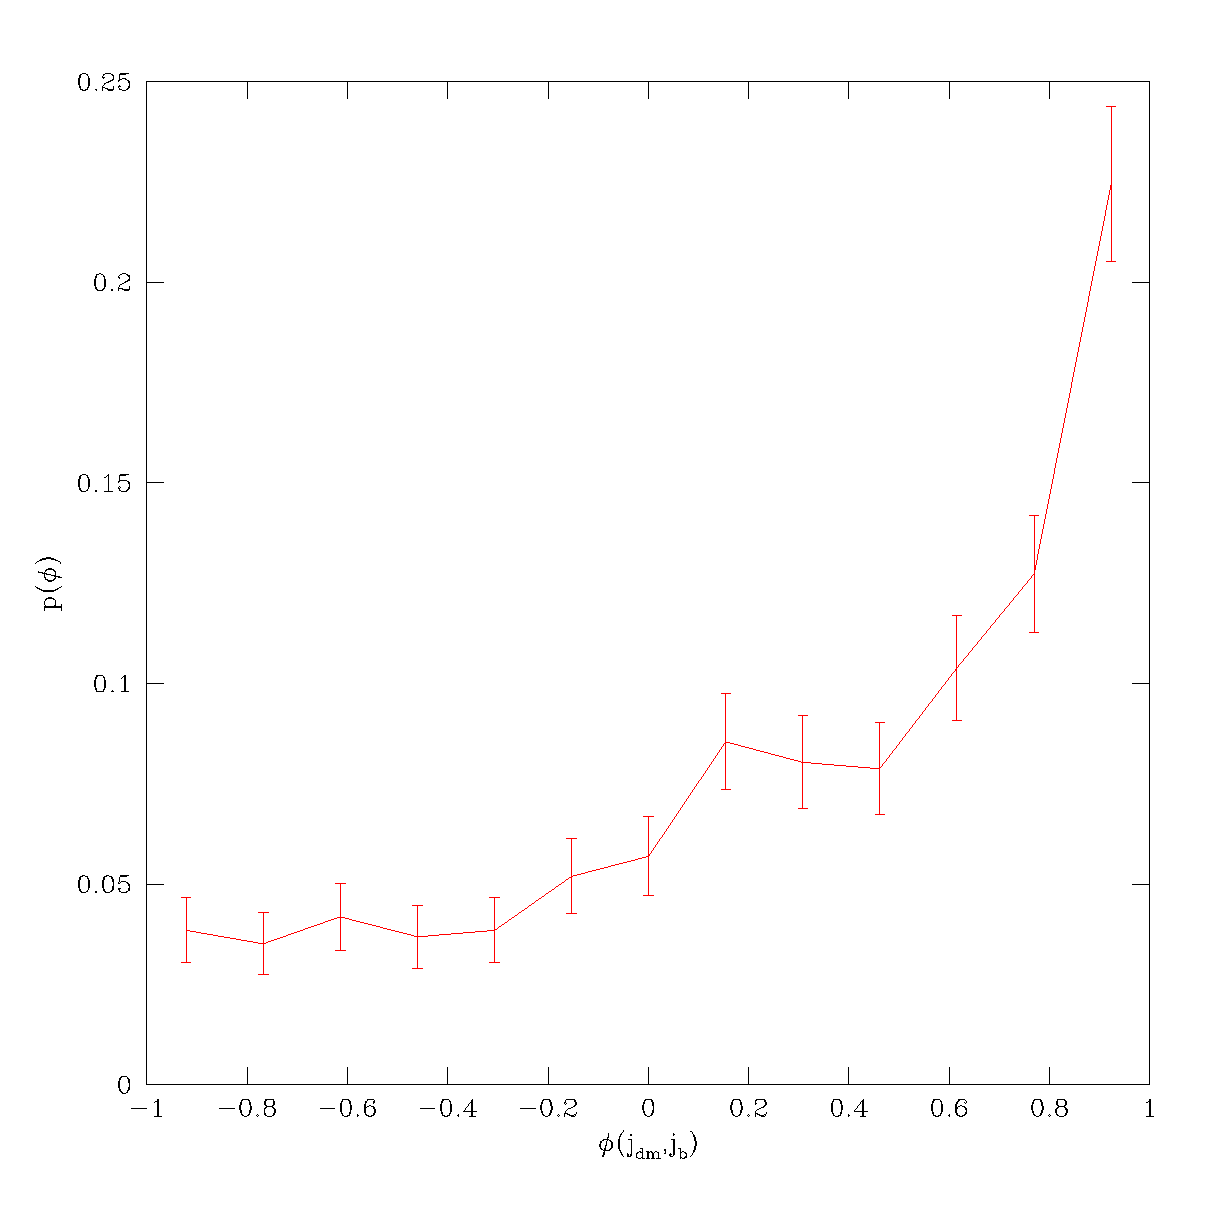
\includegraphics[width=0.45\textwidth]{fig/j_db/out.eps}
  \end{center}

  \caption{ \label{fig:j_db} Distribution of angle $\phi$ between the angular
    momentum axis of dark matter and baryonic halo components.}
\end{figure}
%
%
We find that the angular momenta of the dark matter halos and the star
constituents do well correlate with each other, with a median angle of
$59^\circ$. Gas angular momentum is inclined by a median $76^\circ$ with
respect to dark matter. To compare with observations, we need to add up stars
and gas as baryonic, visible parts. The angular momentum disalignment of
$\phi(\mathbf{j}_{\rm dm},\mathbf{j}_{\rm bary})$ is shown in figure
\ref{fig:j_db}. There are only little negative values for $\phi$, which
contribute all less than the value for an isotropic distribution of $7.7\%$,
indicating that counterrotation is suppressed.

%
%%%fig:j_dgs_r
%
\begin{figure}
  \begin{center}
    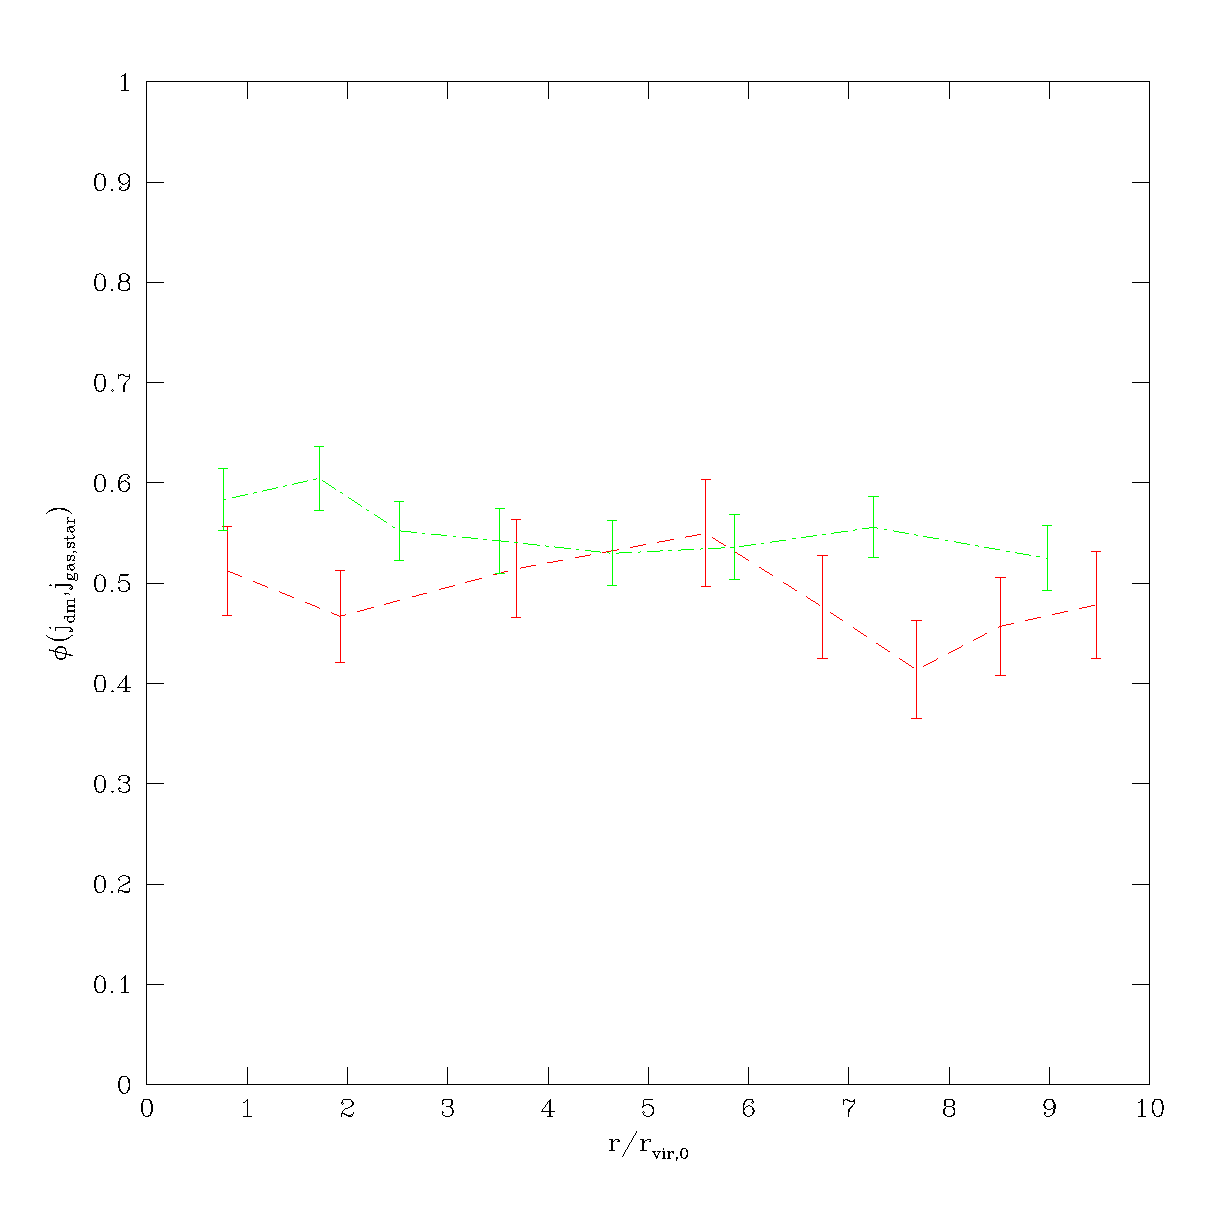
\includegraphics[width=0.45\textwidth]{fig/j_dgs_r/out.eps}
  \end{center}

  \caption{ \label{fig:j_dgs_r} Correlation between $\mathbf{j}_{\rm dm}$ and
    $\mathbf{j}_{\rm gas}$ in red, $\mathbf{j}_{\rm star}$ in green as
    function of distance to cluster center.}
\end{figure}
%
%
We searched for a dependence of this alignment on radial distance and mass:
Figure \ref{fig:j_dgs_r} shows the alignment as function of $r/r_{\rm vir}$,
where $r$ is the distance from the host halo and $r_{\rm vir}$ is the virial
radius of the host. The wide range plotted for $r/r_{\rm vir}$ allows to
include halos in the outskirts of the main clusters, which are not assigned a
host halo. One assumes, though, that the influence on alignment drops rapidly
with distance and is practically negligible for $r/r_{\rm vir}>3$.

There is an alignment between $\mathbf{j}_{\rm dm}$ and $\mathbf{j}_{\rm
  star}$ near the host halo, where $r/r_{\rm vir}\approx 1$. This alignment
extends out to $r/r_{\rm vir}=2.5$ for dark matter and stars; gas does not
seem to be aligned as much. It does not show any alignment with significance
over $2\sigma$, independent on radius.

%
%%%fig:j_dgs_m
%
\begin{figure}
  \begin{center}
    \includegraphics[width=0.45\textwidth]{fig/j_dgs_m/out.eps}
  \end{center}

  \caption{ \label{fig:j_dgs_m} Correlation between $\mathbf{j}_{\rm dm}$ and
    $\mathbf{j}_{\rm gas}$ in red, $\mathbf{j}_{\rm star}$ in green as
    function of halo mass.}
\end{figure}
%
%
As shown in figure \ref{fig:j_dgs_m} -- where we adjusted the mass bin size to
include the same number of halos -- we find a trend for stronger alignment
between angular momentum of stars and dark matter for increasing mass; the
same conclusion cannot be drawn for gas, which is not significantly different
from an isotropic distribution. A small enhancement in the very low and high
mass regime is observed, though, indicating that halos with low gas fraction
follow the overall behavior a little more likely than halos with a relatively
high gas fraction.
%
%
\subsection{Tidal Field}
%
%%%fig:tea_dgs
%
\begin{figure}
  \begin{center}
    \includegraphics[width=0.45\textwidth]{fig/tea_dgs/out.eps}
  \end{center}

  \caption{ \label{fig:tea_dgs} Correlation between $\mathbf{t}_1$, tidal
    field eigenvector corresponding to $\tau_1$, and main inertia axis
    $\mathbf{e}_1$. The smoothing scale for the tidal field is $1\,h^{-1}{\rm
      Mpc}$.}
\end{figure}
%
%
%%%fig:tj_dgs
%
\begin{figure}
  \begin{center}
    \includegraphics[width=0.45\textwidth]{fig/tj_dgs/out.eps}
  \end{center}

  \caption{ \label{fig:tj_dgs} Correlation between $\mathbf{t}_1$ and angular
    momentum $\mathbf{J}$ for a smoothing scale of $1\,h^{-1}{\rm Mpc}$ }
\end{figure}
%
%
We were able to reproduce the expected correlation between different
components of the tidal field eigenvectors and the inertia axes,
cf. \cite{Porciani2002b}. One of the strongest correlations is shown in figure
\ref{fig:tea_dgs}, where the tidal field smoothed over $1\,h^{-1}{\rm Mpc}$
and evaluated at the position of each halo is compared with the main inertia
axis.

We found a similar correlation between tidal field and angular momentum,
illustrated in figure \ref{fig:tj_dgs}. This is no surprise, given that $J$
points roughly in the direction of a characteristic inertial eigenvector --
which in turn is supported by e.g. \cite{Croft2008} with a detected median
angle of $48.3^\circ$.
%
%
\section{Summary and Discussion}
\label{chap:disc}
%
We began by calculating the differential subhalo mass function and found it
consistent with a power law of slope $-1$.

Next we considered the shape of the galaxies by both the sphericity and the
radial dependence of alignment between the halo constituents inertia axes and
radial vector to the host. Sphericity follows a powerlaw. On small radii the
distribution of the angle between inertia axes and radial vector is not
consistent with an isotropic one, with strong alignment for massive halos in
comparison with smaller ones. Stars are aligned even stronger than the dark
matter in low mass halos, due to their relatively recent rearranging to the
enhanced large scale structure.

Kinematical properties were studied with the spin parameter distribution,
rotation support and alignment of angular momenta. The spin parameter was
found to have a log-normal distribution for all components, with roughly the
same peak position for dark matter and stars and a peak for gas that lies an
order of magnitude higher, indicating more ordered rotation. This is confirmed
by direct measurement of ordered rotation for the three components, where dark
matter shows practically no ordered rotation, while gas is showing a broad
distribution of rotation support, mostly in the ordered rotation
regime. Angular momentum vectors of stars and dark matter do show then
preferrred alignment relative to each other, while gas is less well correlated
with dark matter. The baryonic part of the halo does not counterrotate. The
alignment is strongest in the near vicinity of the host or cluster halo.

Correlations between the main tidal field eigenvector and main inertia axis as
well as angular momentum vector are shown, they resemble the one for the
distribution between dark matter and baryonic angular momentum axis.
%
% further: higher resolution, AGN feedback
The computations of the angular momentum of gas and star components do suffer
uncertainties due to low particle numbers; higher resolution is needed to fix
these. AGN feedback should be included as well in later work to constrain
overcooling.
% further: hot/cold gas
It would be interesting for further investigations to divide the gas component
into cold and hot gas or gas in the proximity of stars and gas farther away,
allowing to condense the main contributions.
% further: evolution
The framework developed so far enables to follow the evolution of the
properties from big structures at early times down to small structures at late
times. In future work this redshift dependence shall be included in the
analysis. The evolution of the most relevant scales for the smoothing of the
tidal field would allow insight into which part of the angular momentum is
generated at which epoch.
%
\section*{Acknowledgements}
%
We would like to thank Steffen Knollmann and Alexander Knebe for making the
{\sc Ahf} code publicly available. PS is grateful for stimulating discussions
with Romain Teyssier. All simulations presented are a subset of the {\sc
  Tarkin} simulation set performed at the University of Padova. This work
makes use of the {\sc Nasa} Astrophysics Data System.
%
%
\section{Appendix: Numerical Robustness}
%
Both {\sc Amiga} and our code were used to calculate the key features. Compared to each other, they show a very close agreement for the vast majority
of the halos.
%
We do see however, that our virial mass is off by a mean $8.5\%$ of the total
mass attributed to a halo. This is explained partly by the shift between the
centers of the halos -- center of mass or most bound particle -- and the fact
that we use another measure of the virial radius $R_{vir}$, which is used for
calculations of $M_{vir}$ and therefore angular momentum, spin parameter,
shape parameters and $\Sigma/V$ as well.
%
%%%fig:sigmav_ahf_hp
%
\begin{figure}
  \begin{center}
    \includegraphics[width=0.45\textwidth]{fig/sigmav_ahf_hp/out.eps}
  \end{center}

  \caption{ \label{fig:sigmav_ahf_hp} $\Sigma/V$ distribution as given from
    {\sc Ahf} (in blue) and our own procedure (in red).}
\end{figure}
%
%
Another possibility for mismatches comes from the fact that we restrict
ourselves to halos with a minimum number of particles which is more
restrictive than the 30 particles from {\sc Ahf}. An example comparison of the
value for $\Sigma/V$ calculated from all particles is given by figure
\ref{fig:sigmav_ahf_hp}: The bias towards galaxies with a minimum gas fraction
and the fact that gas shows higher rotation support induces a higher fraction
of highgly rotationally supported systems in the left, while restriction to
halos with more dark matter enhances the abundance of low rotationally
supported systems with respect to the unbiased distribution from {\sc Ahf}
values.
%
%
\section{Appendix: Filament Simulation}
The filament simulation was run on a box with size $10\,{\rm Mpc}$, in
a cosmology with $H_0=70.3\,{\rm km}\,{\rm s}^{-1}\,{\rm Mpc}^{-1}$,
$\Omega_M=0.276$, $\Omega_\Lambda=0.724$, $\Omega_B=0.045$. It was
started at TODO and run until $z=0.05$. See \cite{Hahn2010} for a
detailed description.


%%% end of content
%
% sample figure inclusion statements
%
% \begin{figure}
%   \begin{center}
%     \includegraphics[width=0.45\textwidth]{fig/label}
%   \end{center}
%   \caption{\label{fig:label}small figure, width one column}
% \end{figure}
%
% spanning two columns
%
% \begin[ht]{figure*}
%   \begin{center}
%     \hspace{1cm}
%     \includegraphics[width=0.85\textwidth]{fig/label}
%   \end{center}
%   \caption{\label{fig:label}big figure, width one page}
% \end{figure*}
%
%
\bibliography{main}
%
\label{lastpage}
\end{document}
